%iffalse
\documentclass[journal]{IEEEtran}
\usepackage[a5paper, margin=10mm]{geometry}
%\usepackage{lmodern} % Ensure lmodern is loaded for pdflatex
\usepackage{tfrupee} % Include tfrupee package


\setlength{\headheight}{1cm} % Set the height of the header box
\setlength{\headsep}{0mm}     % Set the distance between the header box and the top of the text


%\usepackage[a5paper, top=10mm, bottom=10mm, left=10mm, right=10mm]{geometry}

%
\setlength{\intextsep}{10pt} % Space between text and floats

\makeindex


\usepackage{cite}
\usepackage{amsmath,amssymb,amsfonts,amsthm}
\usepackage{algorithmic}
\usepackage{graphicx}
\usepackage{textcomp}
\usepackage{xcolor}
\usepackage{txfonts}
\usepackage{listings}
\usepackage{enumitem}
\usepackage{mathtools}
\usepackage{gensymb}
\usepackage{comment}
\usepackage[breaklinks=true]{hyperref}
\usepackage{tkz-euclide} 
\usepackage{listings}
\usepackage{multicol}
\usepackage{xparse}
\usepackage{gvv}
%\def\inputGnumericTable{}                                 
\usepackage[latin1]{inputenc}                                
\usepackage{color}                                            
\usepackage{array}                                            
\usepackage{longtable}                                       
\usepackage{calc}                                             
\usepackage{multirow}                                         
\usepackage{hhline}                                           
\usepackage{ifthen}                                               
\usepackage{lscape}
\usepackage{tabularx}
\usepackage{array}
\usepackage{float}
\usepackage[justification=centering]{caption}


\newtheorem{theorem}{Theorem}[section]
\newtheorem{problem}{Problem}
\newtheorem{proposition}{Proposition}[section]
\newtheorem{lemma}{Lemma}[section]
\newtheorem{corollary}[theorem]{Corollary}
\newtheorem{example}{Example}[section]
\newtheorem{definition}[problem]{Definition}
\newcommand{\BEQA}{\begin{eqnarray}}
\newcommand{\EEQA}{\end{eqnarray}}

\theoremstyle{remark}


\begin{document}
\bibliographystyle{IEEEtran}
\onecolumn

\title{Naval Architecture and Marine Engineering}
\author{EE25BTECH11026-Harsha}
\maketitle

\renewcommand{\thefigure}{\theenumi}
\renewcommand{\thetable}{\theenumi}
\setcounter{secnumdepth}{0}
\subsection{\underline{\textbf{General Aptitude (G.A)}}}
\subsubsection{\underline{Q.1 \text{-} Q.5 Carry ONE mark Each}}
\setlength{\parskip}{1em}


\begin{enumerate}
 \item If '$\rightarrow$' denotes an increasing order of intensity, then the meaning of the words
\(\text{dry} \rightarrow \text{arid} \rightarrow \text{parched}\) is analogous to
\(\text{diet} \rightarrow \text{fast} \rightarrow \underline{\hspace{2cm}}\).
Which one of the given options is appropriate to fill in the blank? 
\begin{multicols}{4}
\begin{enumerate}
        \item starve
        \item reject
        \item feast
        \item deny 
\end{enumerate}
\end{multicols}
\end{enumerate}

\begin{enumerate}[itemsep=1em]
\setcounter{enumi}{1}

\item For two distinct non-zero real variables $x$ and $y$ such that $x + y$ is proportional to $x - y$, find the value of $\tfrac{x}{y}$.


\begin{enumerate}[ leftmargin=2.5em, labelsep=0.5em, itemsep=0.5em]
    \item depends on \(xy\) and on \(x\) and not on \(y\)
    \item depends only on \(y\) and not on \(x\)
    \item depends only on \(x\) and not on \(y\)
    \item is a constant \\
\end{enumerate}

\end{enumerate}

\begin{enumerate}[itemsep=1em]
\setcounter{enumi}{2}

\item Consider the following sample of numbers\:
    $9$, $18$, $11$, $14$, $15$, $17$, $10$, $69$, $11$, $13$
    The median of the sample is 
\begin{multicols}{4}
\begin{enumerate}
        \item $13.5$
        \item $14$
        \item $11$
        \item $18.7$\\
    \end{enumerate}
\end{multicols}
\end{enumerate}


 \begin{enumerate}[itemsep=1em]
\setcounter{enumi}{3}
\item The number of coins of denominations \rupee1, \rupee5 and \rupee10 that a person has is in the ratio 5:3:13. Of the total amount,the percentage of money in \rupee 5 coins is
\begin{multicols}{4}
\begin{enumerate}
        \item $21\%$
        \item $14\tfrac{2}{7}\%$
        \item $10\%$
        \item $30\%$\\
    \end{enumerate}
\end{multicols}
\end{enumerate}

\newpage
\vspace*{0.25cm}



\begin{enumerate}[itemsep=1em]
\setcounter{enumi}{4}
\item For positive non-zero real variables $p$ and $q$, if 
\begin{align*}
    \log \left( p^2 + q^2 \right) &= \log p + \log q + 2 \log 3,
\end{align*}
then, the value of 
\[
    \frac{p^4 + q^4}{p^2 q^2} \quad is
\]
\begin{multicols}{4}
\begin{enumerate}
        \item $79$
        \item $81$
        \item $9$
        \item $83$
    \end{enumerate}
\end{multicols}
\end{enumerate}
\vspace*{0.5cm}



\subsubsection{\underline{Q.6 \text{-} Q.10 Carry TWO marks Each}}



\begin{enumerate}
\setcounter{enumi}{5}

\item In the given text, the blanks are numbered (i)-(iv).Select the best match for all the blanks. 
\setlength{\parskip}{1em}


Steve was advised to keep his head \underline{\makebox[2cm]{(i)}} before heading \underline{\makebox[2cm]{(ii)}} to bat;  
for, while he had a head \underline{\makebox[2cm]{(iii)}} batting, he could only do so with a cool head\underline{\makebox[2cm]{(iv)}} his shoulders.

\begin{enumerate}[leftmargin=2.5em, labelsep=0.5em, itemsep=0.5em]
    \item (i) down \quad (ii) down \quad (iii) on \quad (iv) for
    \item (i) on \quad (ii) down \quad (iii) for \quad (iv) on
    \item (i) down \quad (ii) out \quad (iii) for \quad (iv) on
    \item (i) on \quad (ii) out \quad (iii) on \quad (iv) for
\end{enumerate}
\end{enumerate}

\begin{enumerate}[itemsep=1em]
\setcounter{enumi}{6}

\item A rectangular paper sheet of dimensions $54\ \text{cm} \times 4\ \text{cm}$ is taken. The two longer edges of the sheet are joined together to create a cylindrical tube. A cube whose surface area is equal to the area of the sheet is also taken.  

Then, the ratio of the volume of the cylindrical tube to the volume of the cube is:
\begin{multicols}{4}
\begin{enumerate}
      \item 1/$\pi$
      \item 2/$\pi$
      \item 3/$\pi$
      \item 4/$\pi$
\end{enumerate}
\end{multicols}
\end{enumerate}

\begin{enumerate}[itemsep=1em]
\setcounter{enumi}{7}

\newpage
\vspace*{0.25cm}

\item The pie chart presents the percentage contribution of different macro nutrients to a typical $2000$ kcal diet of a person.
\begin{figure}[H]
    \centering
    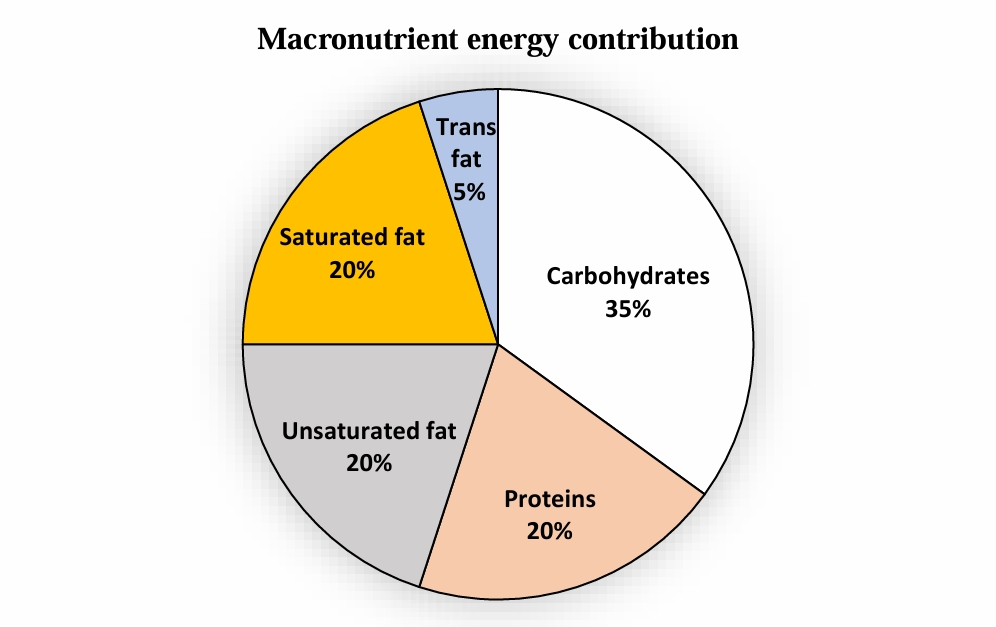
\includegraphics[width=0.5\columnwidth]{figs/fig-1.jpeg}
    \caption*{Fig-1: Macro nutrient energy contribution}
    \label{fig-1}
\end{figure}
The typical energy density (kcal/g) of these macro nutrients is given in the table.  

\begin{table}[h]
\centering
\begin{tabular}{|c|c|} 
\hline
\textbf{Macronutrient} & \textbf{Energy Density (kcal/g)}\\ 
\hline
Carbohydrates & $4$\\ \hline
Proteins & $4$\\ \hline
Unsaturated fat & $9$\\ \hline
Saturated fat & $9$\\ \hline
Trans fat & $9$\\ \hline
\end{tabular}
\end{table}
The total fat (all three types), in grams, this person consumes is 
\begin{multicols}{4}
\begin{enumerate}
         \item $44.4$
         \item $77.8$
         \item $100$
         \item $3600$
    \end{enumerate}
\end{multicols}

\end{enumerate}



\begin{enumerate}[itemsep=1em]
\setcounter{enumi}{8}
\item A rectangular paper of dimensions $20\ \text{cm} \times 8\ \text{cm}$ is folded three times. Each fold is made along the line of symmetry, which is perpendicular to its longer edge. 
The perimeter of the final folded sheet (in cm) is:
\begin{multicols}{4}
\begin{enumerate}
       \item $18$
       \item $24$
       \item $20$
       \item $21$

\end{enumerate}
\end{multicols}
\end{enumerate}

\newpage
\vspace*{0.25cm}

\begin{enumerate}[itemsep=1em]
\setcounter{enumi}{9}
\item The least number of squares to be added in the figure to make AB a line of symmetry is
\begin{figure}[H]
    \centering
    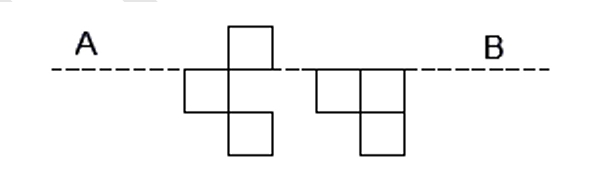
\includegraphics[width=0.5\textwidth]{figs/fig-2.jpeg}
    \caption*{Fig-2}
    \label{fig-2}
\end{figure}
\begin{multicols}{4}
\begin{enumerate}
           \item $6$
           \item $4$
           \item $5$
           \item $7$

\end{enumerate}
\end{multicols}
\end{enumerate}



\subsubsection{\underline{Q.11\text{-}Q.35 Carry ONE Mark each}}

\begin{enumerate}[itemsep=1em]
\setcounter{enumi}{10}
\item The value of the contour integral $\oint \frac{dz}{2z - z^2}$ along the circle $\lvert z \rvert = 1$, oriented in the counterclockwise sense, is:
\begin{multicols}{4}
\begin{enumerate}
        \item $\pi$i
        \item $0$
        \item $2\pi$i
        \item $4\pi$i
\end{enumerate}
\end{multicols}

\end{enumerate}

\begin{enumerate}[itemsep=1em]
\setcounter{enumi}{11}
\item The tangent plane to the surface $x^2 + y^2 + z = 9$ at the point $(1, 2, 4)$ is:

\begin{enumerate}[leftmargin=2.5em, labelsep=0.5em, itemsep=0.5em]
        \item $2x+4y+z=14$
        \item $4x+2y+z=12$
        \item $x+4y+2z=17$
        \item $4x+y+2z=14$
\end{enumerate}
\end{enumerate}



\begin{enumerate}[itemsep=1em]
\setcounter{enumi}{12}
\item The value of the line integral $\oint x^2 \, dx + 2x \, dy$ along the ellipse $4x^2 + y^2 = 4$ oriented in the counterclockwise sense is:
\begin{multicols}{4}
\begin{enumerate}
        \item $\pi$
        \item $2\pi$
        \item $4\pi$
        \item $8\pi$
\end{enumerate}
\end{multicols}

\end{enumerate}

\newpage
\vspace*{0.25cm}

\begin{enumerate}[itemsep=1em]
\setcounter{enumi}{13}
\item The system of linear equations 
\[
x + 2y + 3z = 4
\]
\[
2x - y - 2z = a^2
\]
\[
- x - 7y - 11z = a
\]
has a solution if the values of $a$ are:
\begin{multicols}{4}
\begin{enumerate}
        \item $-1\quad and\;-5$
        \item $-2\quad and\quad3$
        \item $-5\quad and\quad1$
        \item $-3\quad and\quad4$
\end{enumerate}
\end{multicols}

\end{enumerate}

\begin{enumerate}[itemsep=1em]
\setcounter{enumi}{14}
\item A ship with a standard right-handed coordinate system has positive \(x, y, z\) axes respectively pointing towards bow, starboard, and down as shown in the figure. If the ship takes a starboard turn, then the drift angle, sway velocity, and the heel angle of the ship for a steady yaw rate respectively are
\begin{figure}[H]
    \centering
    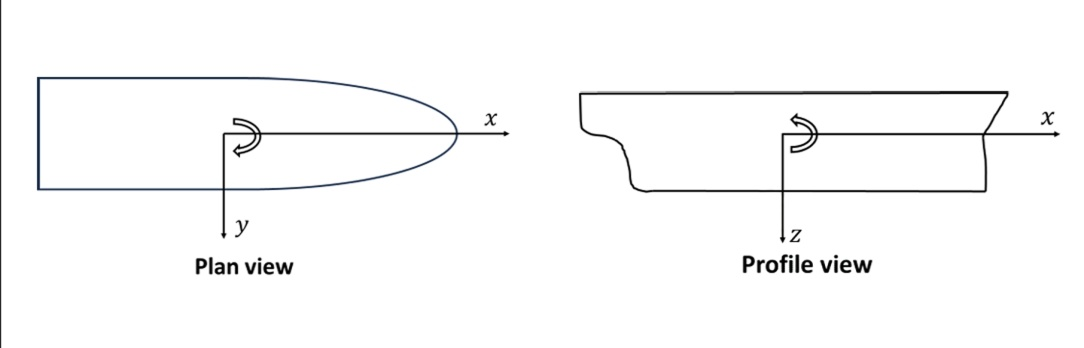
\includegraphics[width=0.5\textwidth]{figs/fig-3.jpeg}
    \caption*{Fig-3}
    \label{fig-3}
\end{figure}
\begin{enumerate}[leftmargin=2.5em, labelsep=0.5em, itemsep=0.5em]
        \item positive, negative and positive
        \item negative, positive and positive
        \item negative, positive and negative
        \item positive, negative and negative
\end{enumerate}

\end{enumerate}

\newpage
\vspace*{0.25cm}

\begin{enumerate}[itemsep=1em]
\setcounter{enumi}{15}
\item A ship with controls fixed, is modeled as a two degrees of freedom system. For the linear maneuvering equations of motion for coupled sway and yaw, if the derived eigenvalues are real and negative, then the ship must possess 
\begin{enumerate}[leftmargin=2.5em, labelsep=0.5em, itemsep=0.5em]
      \item positional motion stability
      \item directional stability
      \item straight line stability
      \item both directional and positional motion stabilities
\end{enumerate}

\end{enumerate}

\begin{enumerate}[itemsep=1em]
\setcounter{enumi}{16}
\item Which of the following cooling systems is used in large marine diesel engines?
\begin{enumerate}[ leftmargin=2.5em, labelsep=0.5em, itemsep=0.5em]
      \item Thermosyphon
      \item Forced coolant circulation
      \item Evaporative
      \item Air circulation
\end{enumerate}
\end{enumerate}

\begin{enumerate}[itemsep=1em]
\setcounter{enumi}{17}
\item Which one of the following reduces the ratio of vibratory response amplitude to the forcing amplitude, in large stationary engine shaft design?
\begin{enumerate}[leftmargin=2.5em, labelsep=0.5em, itemsep=0.5em]
      \item Reduction in axial vibrations of the rotating shaft 
      \item Increase in the fundamental frequency of the rotating shaft
      \item Decrease in the rotational speed of shaft  
      \item Operating the shaft at a speed exceeding the critical speed  
\end{enumerate}
\end{enumerate}

\newpage
\vspace*{0.25cm}

\begin{enumerate}[itemsep=1em]
\setcounter{enumi}{18}
\item The GZ curve for a stable ship is shown in the figure, where P is a point of inflection on the curve. Match the labels in \textbf{column 1} with the corresponding descriptions in \textbf{column 2}. 
\begin{figure}[H]
    \centering
    \caption*{Fig-4: GZ curve for a stable ship}
    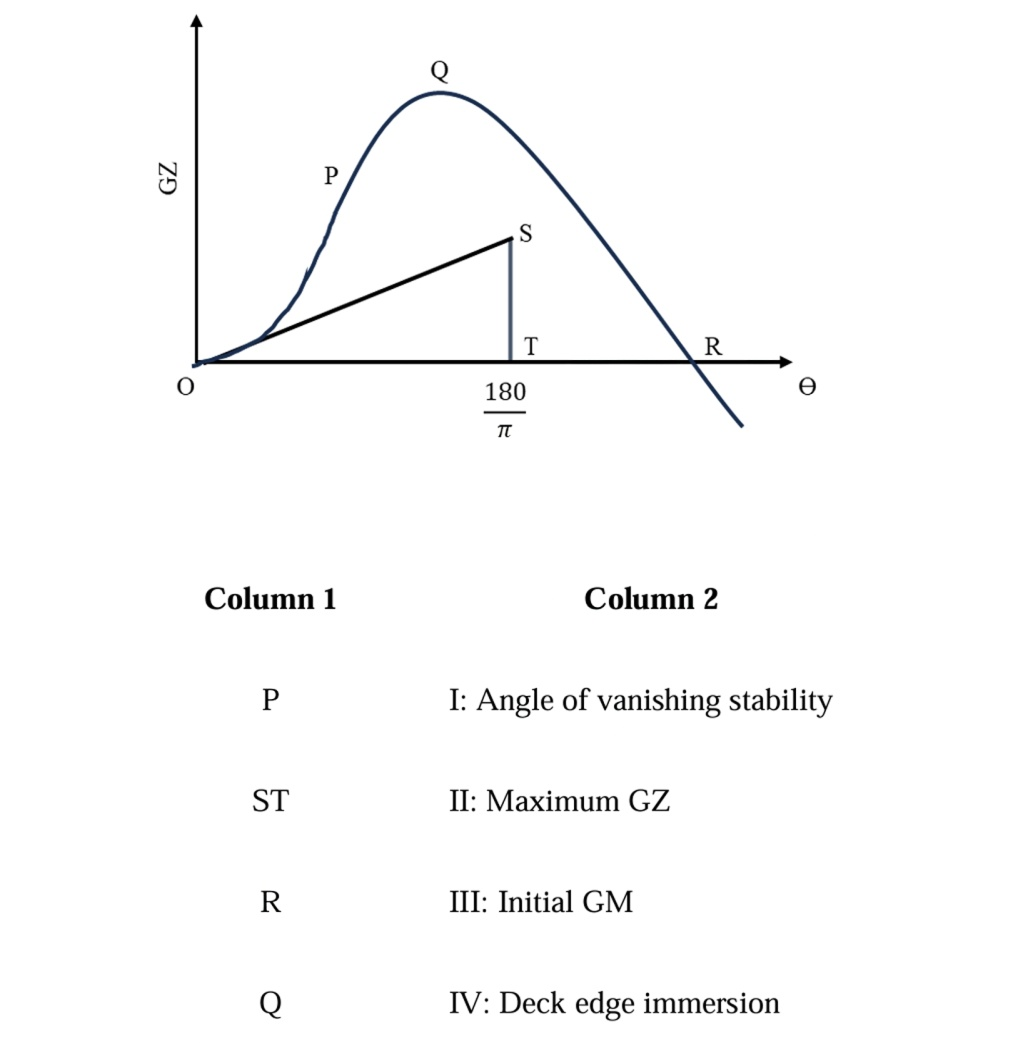
\includegraphics[width=0.5\textwidth]{figs/fig-4.jpeg}
    \label{fig-4}
\end{figure}
\begin{enumerate}[leftmargin=2.5em, labelsep=0.5em, itemsep=0.5em]
      \item R - I; Q - II; ST - III; P - IV 
      \item P - I; Q - II; ST - III; R - IV 
      \item ST - I; Q - II; R - III; P - IV   
      \item R - I; Q - II; P - III; ST - IV  
\end{enumerate}

\end{enumerate}

\begin{enumerate}[itemsep=1em]
\setcounter{enumi}{19}
\item Consider an initially perfectly straight elastic column with pinned supports at both ends. If $E$ is the Young's modulus of the material, $L$ is the length of the column between the supports, and $I$ is the least moment of inertia of the constant cross-sectional area of the column, then the Euler load is given by
\begin{multicols}{4}
\begin{enumerate}
      \item $\frac{\pi^2EI}{L^2}$
      \item $\frac{\pi^2EI}{4L^2}$
      \item $\frac{\pi^2EI}{\sqrt{2}L^2}$  
      \item $\frac{2\pi^2EI}{L^2}$
\end{enumerate}
\end{multicols}
\end{enumerate}

\newpage
\vspace*{0.25cm}

\begin{enumerate}[itemsep=1em]
\setcounter{enumi}{20}
\item For a plane strain problem in the $x$-$y$ plane, it is necessary that 
\begin{enumerate}[leftmargin=2.5em, labelsep=0.5em, itemsep=0.5em]
      \item The normal stress $\sigma_z$ is zero
      \item normal strain $\epsilon_z$ is zero
      \item both the normal stresses $\sigma_x$ and $\sigma_y$ are zero
      \item shear strain $\gamma_{xy}$ is equal to $\frac{(\epsilon_x-\epsilon_y)}{2}$

\end{enumerate}
\end{enumerate}

\begin{enumerate}[itemsep=1em]
\setcounter{enumi}{21}
\item How many independent material constants in solids are required to define isotropic materials? 
\begin{multicols}{4}
\begin{enumerate}
      \item $2$
      \item $3$
      \item $9$  
      \item $21$
\end{enumerate}
\end{multicols}
\end{enumerate}

\begin{enumerate}[itemsep=1em]
\setcounter{enumi}{22}
\item Which one of the following is the mass conservation equation?
\begin{enumerate}[leftmargin=2.5em, labelsep=0.5em, itemsep=0.5em]
    \item $\frac{D}{Dt} \iiint_{V} \rho \, \overrightarrow{v} \cdot \hat{n} \, dV = 0$
    \item $\frac{\partial}{\partial t} \iiint \rho \, dV = 0 $
    \item $-\frac{\partial}{\partial t} \iint_{V} \!\!\int \rho \, dV 
        = \iint_{S} \rho \, \vec{v} \cdot \hat{n} \, dS $ 
    \item  $-\frac{D}{Dt} \iint_{V} \!\!\int \rho \, dV 
  = \iint_{S} \rho \, \vec{v} \cdot \hat{n} \, dS $ 
  
      
\end{enumerate}
\end{enumerate}

\begin{enumerate}[itemsep=1em]
\setcounter{enumi}{23}
\item Identify the type of flow from the time series plots of instantaneous fluid velocity $(u)$ at a point. 
\begin{figure}[H]
    \centering
    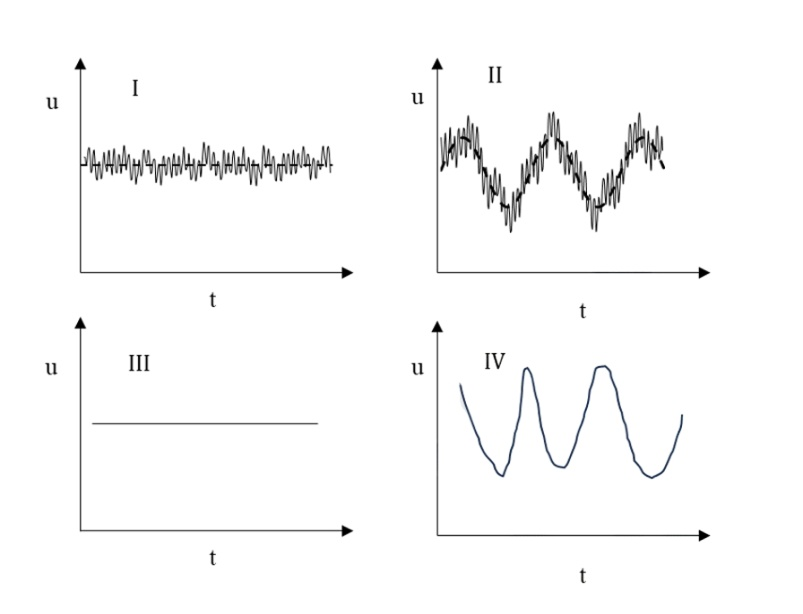
\includegraphics[width=0.5\columnwidth]{figs/fig-5.jpeg}
    \caption*{Fig-5:Time series plots of $(u)$}
    \label{fig-5}
\end{figure}

\newpage
\vspace*{0.25cm}
\begin{enumerate}[leftmargin=2.5em, labelsep=0.5em, itemsep=0.5em]
      \item I - unsteady turbulent flow; II - steady turbulent flow; III - steady laminar flow; IV - unsteady laminar flow 
      \item I - steady turbulent flow; II - unsteady turbulent flow; III - unsteady laminar flow; IV - steady laminar flow 
      \item I - steady turbulent flow; II - unsteady turbulent flow; III - steady laminar flow; IV - unsteady laminar flow 
      \item I - steady turbulent flow; II - unsteady laminar flow; III - unsteady turbulent flow; IV - steady laminar flow 
\end{enumerate}

\end{enumerate}

\begin{enumerate}[itemsep=1em]
\setcounter{enumi}{24}
\item Which of the following hull distortion(s) is/are resisted by a ship's transverse bulkhead?
\begin{enumerate}[leftmargin=2.5em, labelsep=0.5em, itemsep=0.5em]
       \item Racking
       \item Torsion
       \item Longitudinal bending
       \item Horizontal bending
\end{enumerate}
\end{enumerate}

\begin{enumerate}[itemsep=1em]
\setcounter{enumi}{25}
\item Which of the following boiler(s) is/are \textbf{NOT} used in a nuclear propulsion system for ships?
\begin{enumerate}[leftmargin=2.5em, labelsep=0.5em, itemsep=0.5em]
       \item Water tube boiler
       \item Cochran boiler
       \item Double evaporation boiler
       \item Boiled water reactor boiler
\end{enumerate}

\end{enumerate}

\begin{enumerate}[itemsep=1em]
\setcounter{enumi}{26}
\item Which of the following statement(s) is/are correct about strip theory?

\begin{enumerate}[leftmargin=2.5em, labelsep=0.5em, itemsep=0.5em]
       \item It can be used to calculate the surge added mass 
       \item It is a two-dimensional theory 
       \item It can be used to calculate the pitch added mass 
       \item It can be used to calculate the coupled sway, roll and yaw added mass 
\end{enumerate}
\end{enumerate}

\newpage
\vspace*{0.25cm}

\begin{enumerate}[itemsep=1em]
\setcounter{enumi}{27}
\item Consider an ideal Rankine cycle as shown in the figure, where T and S represent the temperature and entropy respectively. The overall efficiency of the cycle can be improved by 
\begin{figure}[H]
    \centering
    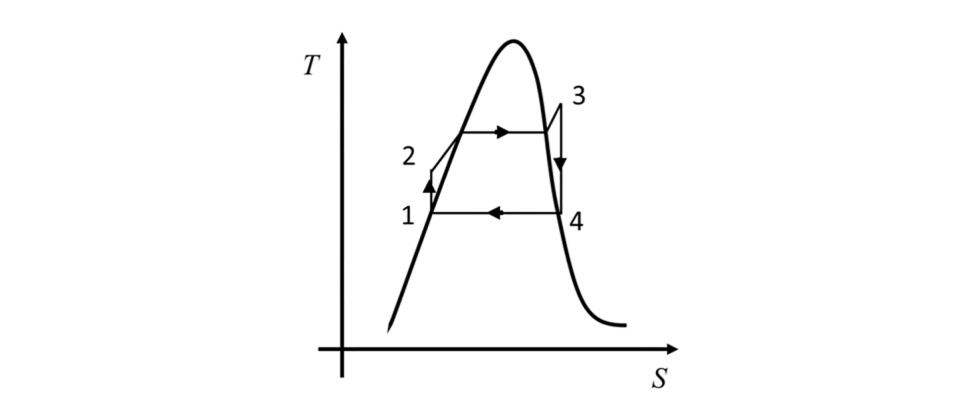
\includegraphics[width=0.5\columnwidth]{figs/fig-6.jpeg}
    \caption*{Fig-6:Rankine cycle}
    \label{fig-6}
\end{figure}

\begin{enumerate}[leftmargin=2.5em, labelsep=0.5em, itemsep=0.5em]
       \item increasing the pressure at which heat is added 
       \item decreasing the pressure at which heat is rejected
       \item employing an intercooler  
       \item super heating the steam  
\end{enumerate}
\end{enumerate}

\begin{enumerate}[itemsep=1em]
\setcounter{enumi}{28}
\item Which of the following statement(s) is/are correct for a thermodynamic closed system?

\begin{enumerate}[ leftmargin=2.5em, labelsep=0.5em, itemsep=0.5em]
       \item The entropy change is positive for a reversible adiabatic process
       \item The entropy change is positive for a reversible cycle 
       \item The entropy change is positive for a reversible isothermal heat addition process  
       \item The entropy change is negative for a reversible isothermal heat rejection process   
\end{enumerate}
\end{enumerate}

\begin{enumerate}[itemsep=1em]
\setcounter{enumi}{29}
\item The arc length of the one arch of the cycloid is given by $x=t-\sin t$ and $y=1-\cos t$ is \underline{\hspace{3cm}}.

\end{enumerate}

\begin{enumerate}[itemsep=1em]
\setcounter{enumi}{30}
\item A $10$ m long pipe with inlet and outlet diameters of $40$ cm and $20$ cm respectively, is carrying an incompressible fluid with a flow rate of $0.04\, m^3/s$. The ratio of the velocity at the outlet to that at the inlet is \underline{\hspace{2cm}}( rounded off to one decimal place) 
\end{enumerate}

\newpage
\vspace*{0.25cm}

\begin{enumerate}[itemsep=1em]
\setcounter{enumi}{31}
\item An $80$ m long barge with rectangular cross-section of $12$ m beam and $4$ m draft floats at even keel. The transverse metacenter (km) above the keel is \underline{\hspace{2cm}} m. 
\end{enumerate}

\begin{enumerate}[itemsep=1em]
\setcounter{enumi}{32}
\item A $100$ m long ship has a cruising speed of $25$ knots. A geometrically similar model of $4$ m length is used for resistance prediction in a towing tank. The corresponding speed of the model is \underline{\hspace{2cm}} knots. 
\end{enumerate}

\begin{enumerate}[itemsep=1em]
\setcounter{enumi}{33}
\item A cube-shaped pontoon with $200$ tonnes of mass placed on it, floats with a freeboard of $1$ m in fresh water. When the mass is removed, the pontoon floats with a freeboard of $3$ m. The length of the pontoon is \underline{\hspace{2cm}} m (rounded off to two decimal places).
\end{enumerate}

\begin{enumerate}[itemsep=1em]
\setcounter{enumi}{34}
\item Consider a fluid between two horizontal parallel flat plates $5$ mm apart as shown in the figure. The top plate of dimensions $0.5\,m \times 2\,m$ is towed with an applied horizontal force F of $0.01$ N, while the infinitely long bottom plate is kept fixed. The horizontal velocity profile between the plates is assumed to be linear. If the 
dynamic viscosity $(\mu)$ of the fluid is $0.89 \times 10^{-3} \quad N-s/m^2$, then the towing velocity of 
the top plate is \underline{\hspace{2cm}} m/s (rounded off to three decimal places).
\begin{figure}[H]
    \centering
    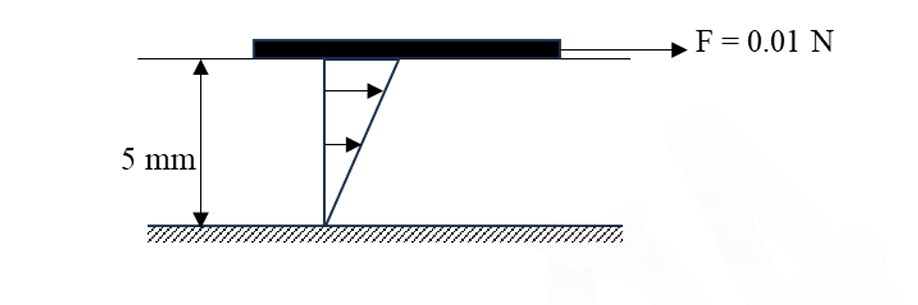
\includegraphics[width=0.5\columnwidth]{figs/fig-7.jpeg}
    \caption*{Fig-7:Fluid between two horizontal parallel flat plates}
    \label{fig-7}
\end{figure}


\end{enumerate}

\newpage
\vspace*{0.25cm}
\subsubsection{\underline{Q.36 - Q.65 Carry TWO marks Each}}

\begin{enumerate}[itemsep=1em]
\setcounter{enumi}{35}
    \item Consider the matrices M=$\begin{myvec}{2&&1 \\ 0 && 2}\end{myvec}$ and N=$\begin{myvec}{1&&0&&0\\1&&2&&0\\1&&1&&0} \end{myvec}$. Which one of the following is true?

\begin{enumerate}[leftmargin=2.5em, labelsep=0.5em, itemsep=0.5em]
       \item $M$ is not diagonalizable but $N$ is diagonalizable 
       \item Both $M$ and $N$ are not diagonalizable
       \item Both $M$ and $N$ are diagonalizable   
       \item $M$ is diagonalizable but $N$ is not diagonalizable 
\end{enumerate}


\end{enumerate}

\begin{enumerate}[itemsep=1em]
\setcounter{enumi}{36}
\item A simply supported beam is subjected to a concentrated moment M at the mid span as shown in the figure. The magnitude of the bending moment at a distance of $L/4$ from the left support A is equal to
\begin{figure}[H]
    \centering
    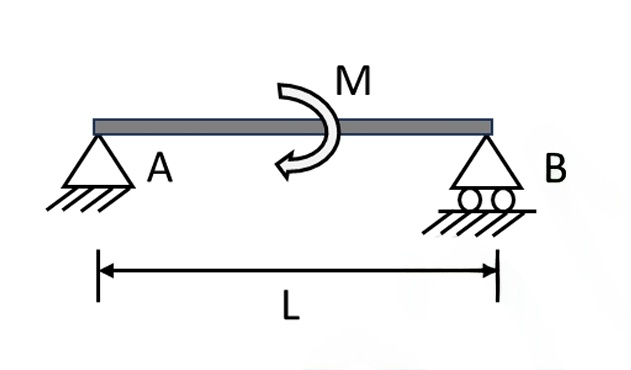
\includegraphics[width=0.5\columnwidth]{figs/fig-8.jpg}
    \caption*{Fig-8:Figure of supporting beam}
    \label{fig-8}
\end{figure}
\begin{multicols}{4}
\begin{enumerate}
       \item $M$
       \item $\frac{ML}{4}$
       \item $\frac{M}{4}$  
       \item $\frac{M}{2}$ 
\end{enumerate}
\end{multicols}

\end{enumerate}

\newpage
\vspace*{0.25cm}

\begin{enumerate}[itemsep=1em]
\setcounter{enumi}{37}
\item Consider a two-dimensional ship section as shown in the figure. About the point O,let the sway added mass components be $a_{22}$ and $a_{24}$ and roll added moment of inertia be $a_{44}$. The clockwise roll angle is considered positive. The roll added mass due to roll, about P which is at a distance $z_p$ above O is given by 
\begin{figure}[H]
    \centering
    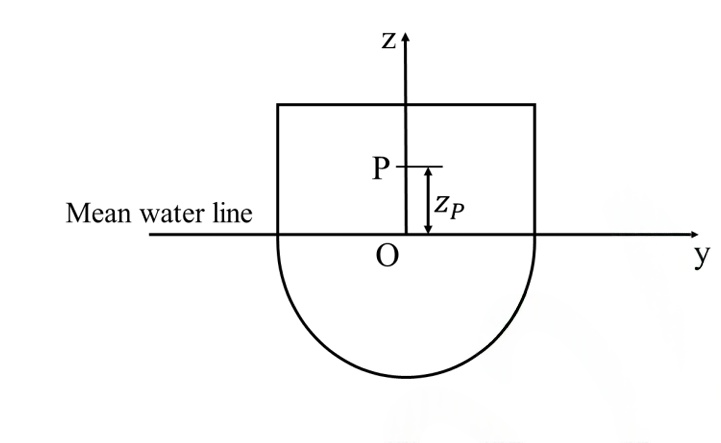
\includegraphics[width=0.5\columnwidth]{figs/fig-9.jpg}
    \caption*{Fig-9: Two dimensional ship section}
    \label{fig-9}
\end{figure}
\begin{multicols}{4}
\begin{enumerate}
       \item $a_{44}-a_{24}z_p$
       \item $a_{44}-a_{22}-a_{24}z_p$
       \item $a_{44}-a_{22}+a_{24}z_p$  
       \item $a_{22}+a_{24}+a_{44}$ 
\end{enumerate}
\end{multicols}


\end{enumerate}

\begin{enumerate}[itemsep=1em]
\setcounter{enumi}{38}
\item A ship with a displacement of $10000$ tonnes has the center of gravity at $4$ m above the keel and $1.5$ m forward of midship. If $2000$ tonnes of cargo is placed at $10$ m 
above the keel and $1.5$m aft of midship, then the new position of the center of gravity is

\begin{enumerate}[ leftmargin=2.5em, labelsep=0.5em, itemsep=0.5em]
       \item $5$m above the keel and $1$m aft of midship 
       \item $6$m above the keel and $1$m forward of midship 
       \item $6$m above the keel and $1$m aft of midship  
       \item $5$m above the keel and $1$m forward of midship 
\end{enumerate}
\end{enumerate}

\begin{enumerate}[itemsep=1em]
\setcounter{enumi}{39}
\item The waterplane area of a ship floating in sea water is $2000\;m^2$. The density of seawater is $1025\;kg/m^3$. If a mass of $246$ tonnes is added to the ship, then the TPC 
(Tonnes Per Centimeter immersion) and increase in draft (in cm) respectively are 
\begin{multicols}{4}
\begin{enumerate}
       \item $20.50$ and $12$
       \item $20$ and $12.3$
       \item $20.50$ and $24$  
       \item $10.25$ and $24.6$ 
\end{enumerate}
\end{multicols}

\end{enumerate}

\newpage
\vspace*{0.25cm}

\begin{enumerate}[itemsep=1em]
\setcounter{enumi}{40}
\item The open water characteristics of a propeller is shown in the figure. Match the labels in \textbf{Column 1} with the corresponding descriptions in \textbf{Column 2}.
\begin{figure}[H]
    \centering
    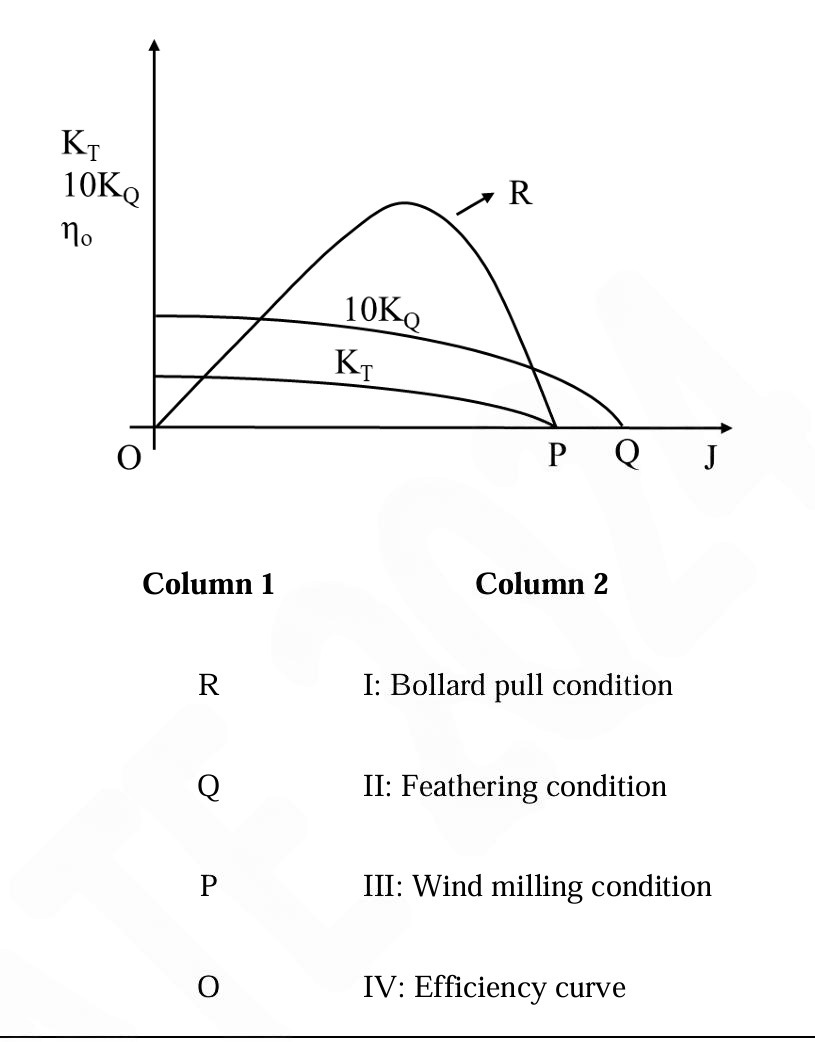
\includegraphics[width=0.5\columnwidth]{figs/fig-10.jpeg}
    \caption*{Fig-10:Open water characteristics of a propeller}
    \label{fig-10}
\end{figure}
\begin{enumerate}[leftmargin=2.5em, labelsep=0.5em, itemsep=0.5em]
      \item O - I; P - II; Q - III; R - IV 
      \item O - I; Q - II; P - III; R - IV 
      \item O - I; R - II; Q - III; P - IV   
      \item P - I; Q - II; O - III; R - IV  
\end{enumerate}

\end{enumerate}

\newpage
\vspace*{0.25cm}

\begin{enumerate}[itemsep=1em]
\setcounter{enumi}{41}
\item Which one of the following p-h plots represents the ideal vapour compression cycle with intercooling?\\  
Here, p and h denote pressure and specific enthalpy respectively. 
\begin{multicols}{4}
\begin{enumerate}
    \item \begin{minipage}[t]{0.2\textwidth}
    \vspace{0pt}
        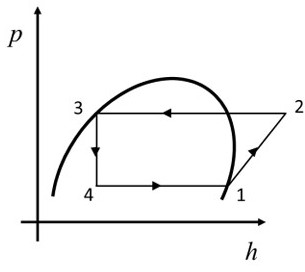
\includegraphics[width=\columnwidth]{figs/fig-11.jpeg}
        \label{fig-11}
    \end{minipage}
    \item \begin{minipage}[t]{0.2\textwidth}
    \vspace{0pt}
        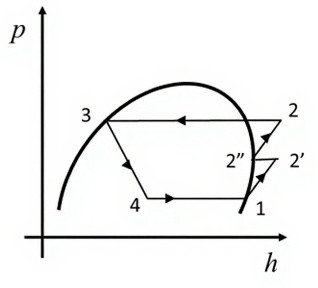
\includegraphics[width=\columnwidth]{figs/fig-12.jpeg}
        \label{fig-12}
    \end{minipage}
    \item \begin{minipage}[t]{0.2\textwidth}
    \vspace{0pt}
        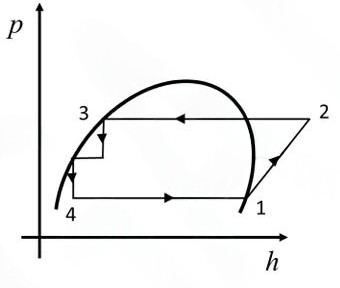
\includegraphics[width=\columnwidth]{figs/fig-13.jpg}
        \label{fig-13}
    \end{minipage}
    \item \begin{minipage}[t]{0.2\textwidth}
    \vspace{0pt}
        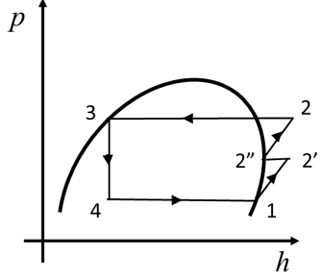
\includegraphics[width=\columnwidth]{figs/fig-14.jpeg}
    \label{fig-14}
    \end{minipage}
\end{enumerate}
\end{multicols}
\end{enumerate}

\begin{enumerate}[itemsep=1em]
\setcounter{enumi}{42}

\item A steel deck plate of a tanker is supported by two longitudinal stiffeners as shown in the figure. The width of the plate is $a$ and its length is $5$ times the width. Assume
that the long edge is simply supported and that the short edge is free. The plate is loaded by a distributed pressure,p=$p_0\sin(\frac{\pi y}{a})$, where $p_0$ is the pressure at $y=a/2$. The flexural rigidity of the plate is $D$. The plate equation is given by

\begin{figure}[H]
    \centering
    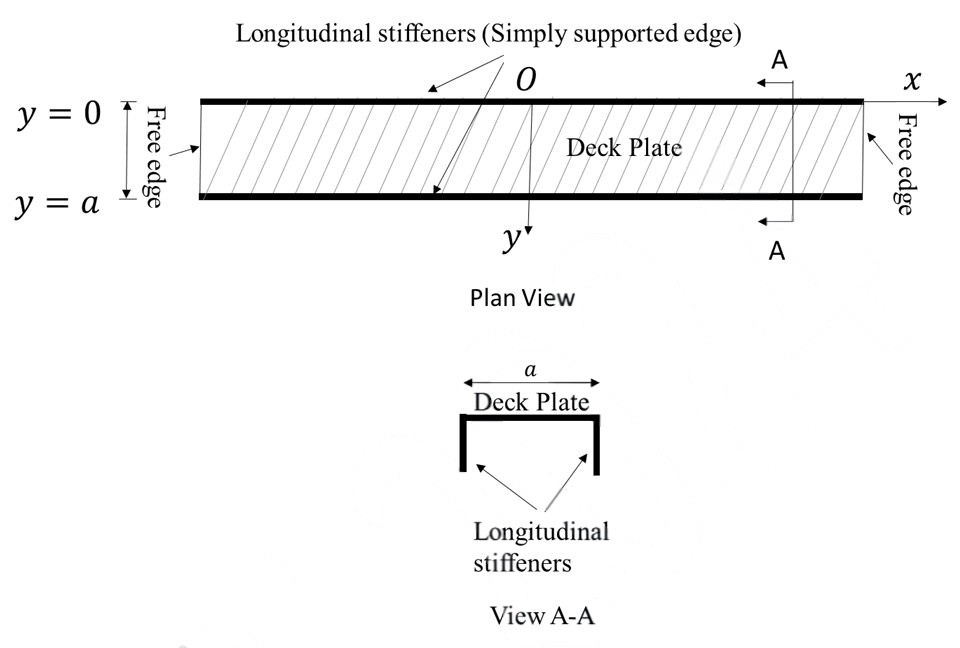
\includegraphics[width=0.5\columnwidth]{figs/fig-15.jpg}
    \caption*{Fig-15:The steel deck plate of the tanker}
    \label{fig-15}
\end{figure}
\begin{multicols}{4}
\begin{enumerate}
    \item $\frac{\partial^4 w}{\partial y^4} = \frac{p_0}{D} \sin\left( \frac{\pi y}{a} \right)$
    \item $\frac{\partial^2 w}{\partial x^2} = \frac{p_0}{D} \sin\left( \frac{\pi y}{a} \right)$
    \item $\frac{\partial^2 w}{\partial x^2} = \frac{p_0}{D} \sin\left( \frac{\pi y}{a} \right)$
    \item $\frac{\partial^4 w}{\partial x^4} = \frac{p_0}{D} \sin\left( \frac{\pi y}{a} \right)$

\end{enumerate}
\end{multicols}
\end{enumerate}

\newpage
\vspace*{0.25cm}

\begin{enumerate}[itemsep=1em]
\setcounter{enumi}{43}
\item Which one of the following psychrometric processes is represented by the line $1$-$2$ in the figure?
\begin{figure}[H]
    \centering
    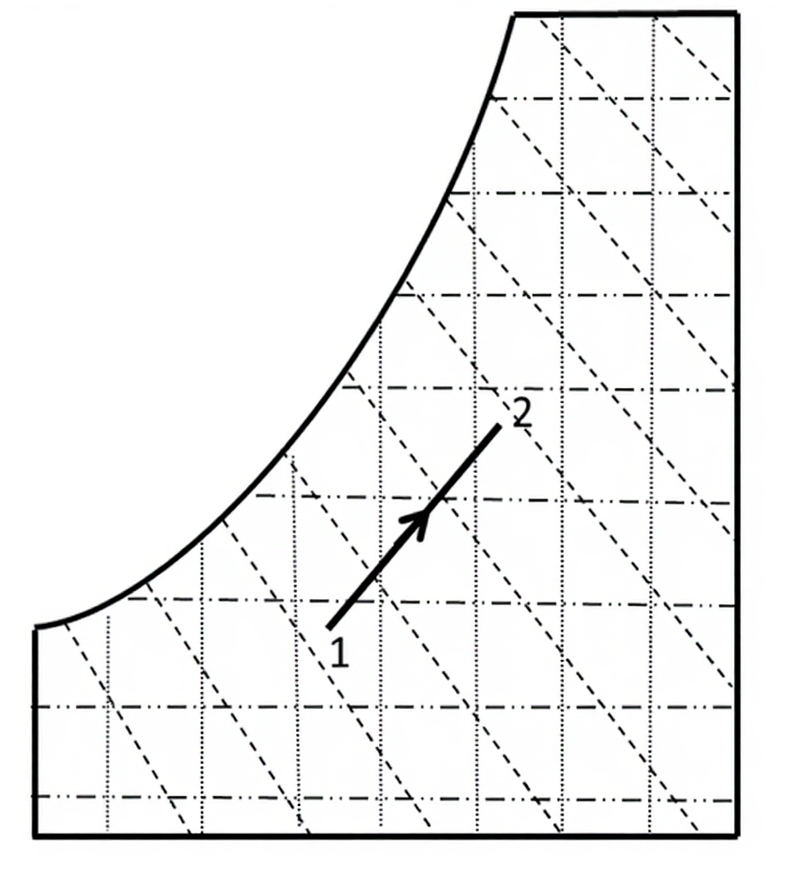
\includegraphics[width=0.4\columnwidth]{figs/fig-16.png}
    \caption*{Fig-16:Psychrometric process graph}
    \label{fig-16}
\end{figure}

\begin{enumerate}[ leftmargin=2.5em, labelsep=0.5em, itemsep=0.5em]
     \item Cooling and humidification 
     \item Cooling and dehumidification
     \item Heating and humidification 
     \item Heating and dehumidification 
\end{enumerate}

\end{enumerate}

\begin{enumerate}[itemsep=1em]
\setcounter{enumi}{44}
\item Consider model testing where $\lambda$ is the prototype to model length scale ratio. Let $v_p$ and $v_m$ denote the corresponding fluid kinematic viscosities. If Froude and Reynolds similarities are maintained between the prototype and model, then which one of the following is correct? 

\begin{multicols}{4}
\begin{enumerate}
     \item $v_m=\lambda^{-3/2}v_p$
     \item $v_m=\lambda^{3/2}v_p$
     \item $v_m=\lambda^{2/3}v_p$
     \item $v_m=\lambda^{-2/3}v_p$
     
\end{enumerate}
\end{multicols}
\end{enumerate}

\newpage
\vspace*{0.25cm}

\begin{enumerate}[itemsep=1em]
\setcounter{enumi}{45}
\item A uniform flow, a point source of strength $+\sigma$  at $(a,0)$ and a point sink of strength $-\sigma$ at $(-a,0)$ are shown in the figure. The velocity potential $\phi$ resulting from the superposition of these flow fields is given by 
\begin{figure}[H]
    \centering
    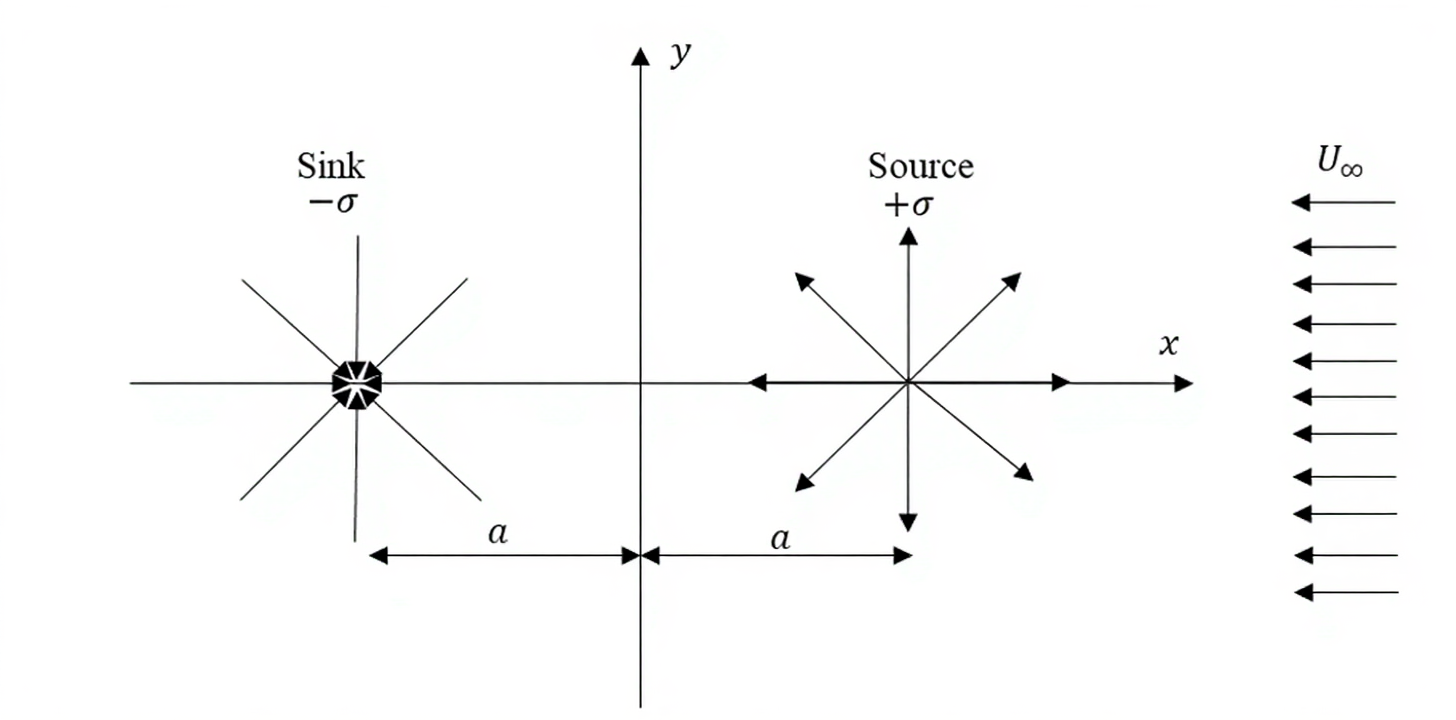
\includegraphics[width=0.4\columnwidth]{figs/fig-17.png}
    \caption*{Fig-17}
    \label{fig-17}
\end{figure}

\begin{enumerate}[leftmargin=2.5em, labelsep=0.5em, itemsep=0.5em]
    \item $\phi = -U_{\infty} x 
+ \frac{\sigma}{2\pi} \ln\sqrt{(x+a)^2 + y^2} 
- \frac{\sigma}{2\pi} \ln\sqrt{(x-a)^2 + y^2}$
    \item $\phi = -U_{\infty} x 
- \frac{\sigma}{2\pi} \ln\sqrt{(x+a)^2 + y^2} 
+ \frac{\sigma}{2\pi} \ln\sqrt{(x-a)^2 + y^2}$
     \item $\phi = U_{\infty} x 
- \frac{\sigma}{2\pi} \ln\sqrt{(x+a)^2 + y^2} 
+ \frac{\sigma}{2\pi} \ln\sqrt{(x-a)^2 + y^2}$
    \item $\phi = U_{\infty} x 
+ \frac{\sigma}{2\pi} \ln\sqrt{(x+a)^2 + y^2} 
- \frac{\sigma}{2\pi} \ln\sqrt{(x-a)^2 + y^2}$

\end{enumerate}



\end{enumerate}

\begin{enumerate}[itemsep=1em]
\setcounter{enumi}{46}
\item In the solution of statically indeterminate problems, Castigliano's second theorem employs the

\begin{enumerate}[ leftmargin=2.5em, labelsep=0.5em, itemsep=0.5em]
    \item principle of virtual work 
    \item virtual displacement method 
    \item virtual force method 
    \item principle of least work
\end{enumerate}

\end{enumerate}

\begin{enumerate}[itemsep=1em]
\setcounter{enumi}{47}
\item Consider the function $f(x,y)=x^4+y^4-4xy+1$.Which of the following is/are correct? 
\begin{enumerate}[ leftmargin=2.5em, labelsep=0.5em, itemsep=0.5em]
    \item The minimum value of $f$ occurs at $(0,0)$  
    \item The point $(0,0)$ is a point of inflection 
    \item $f$ has three critical points 
    \item The minimum value of $f$ is $-1$
\end{enumerate}
\end{enumerate}

\newpage
\vspace*{0.25cm}

\begin{enumerate}[itemsep=1em]
\setcounter{enumi}{48}
\item Consider the $2\pi$ periodic function defined by
\[
f(x) =
\begin{cases}
-1, & \text{if } -\pi < x \le 0, \\
1, & \text{if } 0 < x < \pi.
\end{cases}
\]
Which of the following is/are correct about its Fourier series expansion, $\frac{a_0}{2}+\sum_{n=1}^{\infty}a_n\cos\,nx\,+\,b_n\sin\,nx$?

\begin{enumerate}[leftmargin=2.5em, labelsep=0.5em, itemsep=0.5em]
      \item $a_n=\frac{1}{n}\,\forall\,n=\,1,2,...$
      \item $a_0=0$
      \item $b_n=\frac{4}{n\pi}$ if n is odd
      \item $b_n=-\frac{4}{n\pi}$ if n is even
\end{enumerate}
\end{enumerate}

\begin{enumerate}[itemsep=1em]
\setcounter{enumi}{49}
\item Consider the following momentum equation. Let A, B and C denote the first, second and third term on the left-hand side respectively and, D and E denote the first and second term on the right-hand side respectively. Which of the following statement(s) is/are correct?  
\[
\frac{\partial \mathbf{V}}{\partial t}
+ \nabla \left| \frac{\mathbf{V}^2}{2} \right|
+ \left( \nabla \times \mathbf{V} \right) \times \mathbf{V}
= -\nabla \left( P + \rho g z \right)
+ \mu \nabla^2 \mathbf{V}
\]

\begin{enumerate}[ leftmargin=2.5em, labelsep=0.5em, itemsep=0.5em]
      \item If terms A, C and E vanish, then the flow is irrotational. 
      \item If term A vanishes, then the flow is steady. 
      \item If term D vanishes, then it leads to the Euler's equation. 
      \item If terms A, B, C and E vanish, then it leads to the hydrostatic equation. 
\end{enumerate}
\end{enumerate}

\begin{enumerate}[itemsep=1em]
\setcounter{enumi}{50}
\item Consider the flow past a curved wall as shown in the figure. Which of the following statement(s) is/are correct? 
\begin{figure}[H]
    \centering
    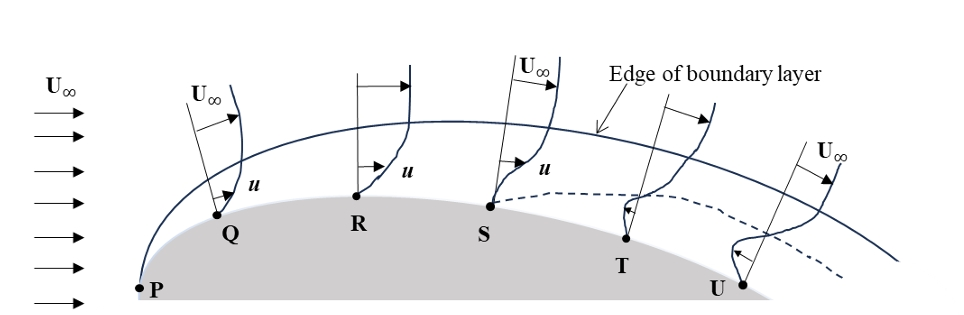
\includegraphics[width=0.6\columnwidth]{figs/fig-18.jpeg}
    \caption*{Fig-18:Flow past the curved wall}
    \label{fig-18}
\end{figure}


\newpage
\vspace*{0.25cm}

\begin{enumerate}[leftmargin=2.5em, labelsep=0.5em, itemsep=0.5em]
      \item P is the separation point.  
      \item Between T and U, the pressure gradient in the streamwise direction at the wall is positive.
      \item U is the stagnation point.  
      \item Between T and U, the streamwise-velocity gradient in the normal direction at the wall is negative. 
\end{enumerate}
\end{enumerate}

\begin{enumerate}[itemsep=1em]
\setcounter{enumi}{51}
\item If $X$ is a Poisson random variable with mean $\mu$=1, then the conditional probability of the event ${X\geq 2}$ given that the event ${X\geq 4}$ has occurred, is
\underline{\hspace{2cm}} (rounded off to two decimal places). 
\end{enumerate}

\begin{enumerate}[itemsep=1em]
\setcounter{enumi}{52}
\item The value of the triple integral $\iiint(xy^2+yz^3)\,dx\,dy\,dz$ over the region given by $-1\leq x\leq 1,\,3\leq y \leq 4,\,0 \leq z \leq 2,$ is \underline{\hspace{2cm}}.
\end{enumerate}

\begin{enumerate}[itemsep=1em]
\setcounter{enumi}{53}
\item A $4$-cylinder, $4$-stroke diesel engine operating at 3000 rpm has a compression ratio r of 12 and cut-off ratio $r_c$ of $2.5$. The temperature rise during the heat addition process is $2400$ K. The efficiency of an air-standard diesel cycle is given by \\$\eta=1\,-\,\frac{1}{r^{\gamma-1}}(\frac{1}{\gamma}\frac{r_c^\gamma-1}{r_c-1})$. Assume the working fluid as air with a mass flow rate of 
$0.05\;kg/s$, $\gamma=1.4$, and $C_p=1.004\;kJ/kg-K$.
The power output of the engine is \underline{\hspace{1cm}}kW (rounded off to the nearest integer)
\end{enumerate}

\begin{enumerate}[itemsep=1em]
\setcounter{enumi}{54}
\item A ship travelling in head seas experiences a bending moment of $200$ MN-m. The ship's cross section is assumed to be a box girder of $30\,m$ beam and $10\,m$ depth with a $10\,mm$ plate thickness. The maximum bending stress is \underline{\hspace{2cm}} MPa 
(rounded off to the nearest integer).
\end{enumerate}

\begin{enumerate}[itemsep=1em]
\setcounter{enumi}{55}
\item A single degree of freedom system has a mass, stiffness and damping of $200\,kg$, $20\,N/m$ and $62$N-s/m respectively. For a forced oscillation system, if the excitation frequency is equal to the undamped natural frequency, then the dynamic 
magnification factor is \underline{\hspace{2cm}} (rounded off to three decimal places). 
\end{enumerate}

\begin{enumerate}[itemsep=1em]
\setcounter{enumi}{56}
\item The wave spectrum and the ship heave Response Amplitude Operator (RAO) are shown in the figure. The variance of the heave motion is \underline{\hspace{2cm}} (rounded off to three decimal places).
\newpage
\vspace*{0.25cm}
\noindent
\begin{minipage}{0.48\columnwidth}
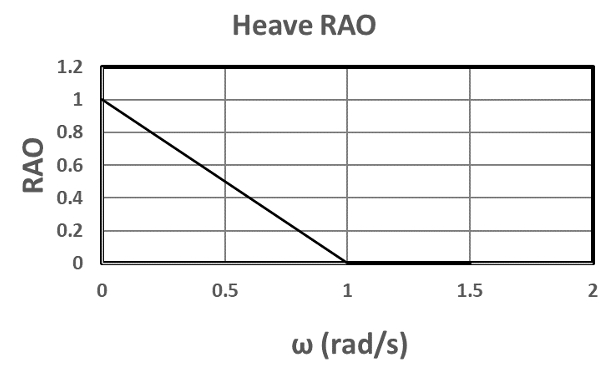
\includegraphics[width=\columnwidth]{figs/fig-19.jpeg}
\captionof*{figure}{fig-19: ship heave RAO}
\end{minipage}\hfill
\begin{minipage}{0.48\columnwidth}
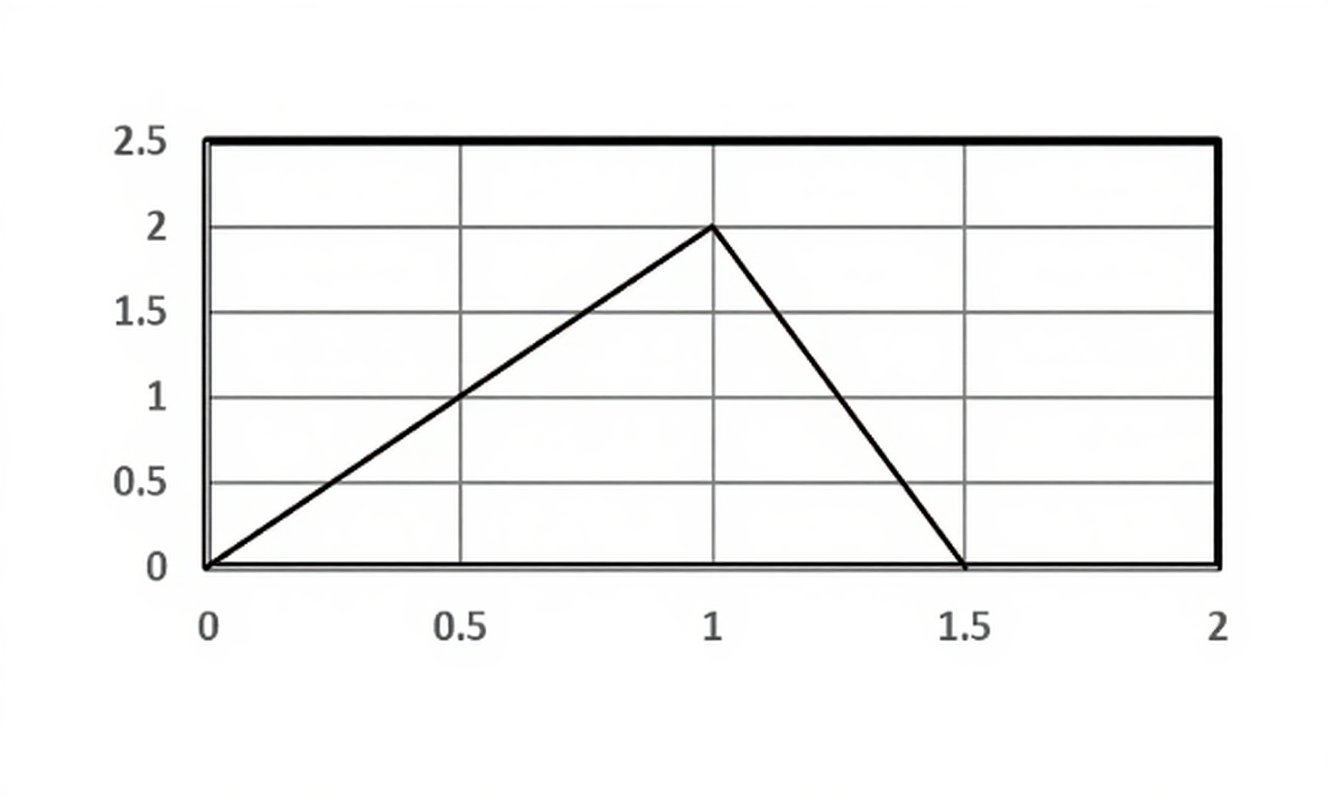
\includegraphics[width=\columnwidth]{figs/fig-20.png}
\captionof*{figure}{fig-20: wave spectrum}
\end{minipage}
\end{enumerate}
\begin{enumerate}[itemsep=1em]
\setcounter{enumi}{57}
\item Consider a thin-walled closed cylindrical steel vessel with an internal pressure of $2\,N/mm^2$. The inner diameter is $1\,m$, and the thickness of the wall is $10\, mm$. The 
hoop stress is \underline{\hspace{2cm}} $N/mm^2$ (rounded off to one decimal place). 
\end{enumerate}

\begin{enumerate}[itemsep=1em]
\setcounter{enumi}{58}
\item A propeller disc of diameter $2\,m$ produces a thrust of $88 \,kN$ while advancing at a speed of $5\,m/s$ in fresh water of density $1000\,kg/m^3$. Based on the axial momentum theory, the propeller efficiency is \underline{\hspace{2cm}} \% (rounded off to one decimal place). 
\end{enumerate}

\begin{enumerate}[itemsep=1em]
\setcounter{enumi}{59}
\item Consider a rectangular plate with in-plane loads. The state of the stress at an arbitrary angle $\theta$ is defined by $\sigma_x$,$\sigma_y$ and $\tau_{xy}$ as shown in the figure. If the principal plane is at $\theta=45\degree$, and the principal stresses are $\sigma_x = 8\,N/mm^2$ and $\sigma_y=3 \,N/mm^2$,then the corresponding $\tau_{xy}=\underline{\hspace{2cm}}\,N/mm^2$.
\begin{figure}[H]
    \centering
    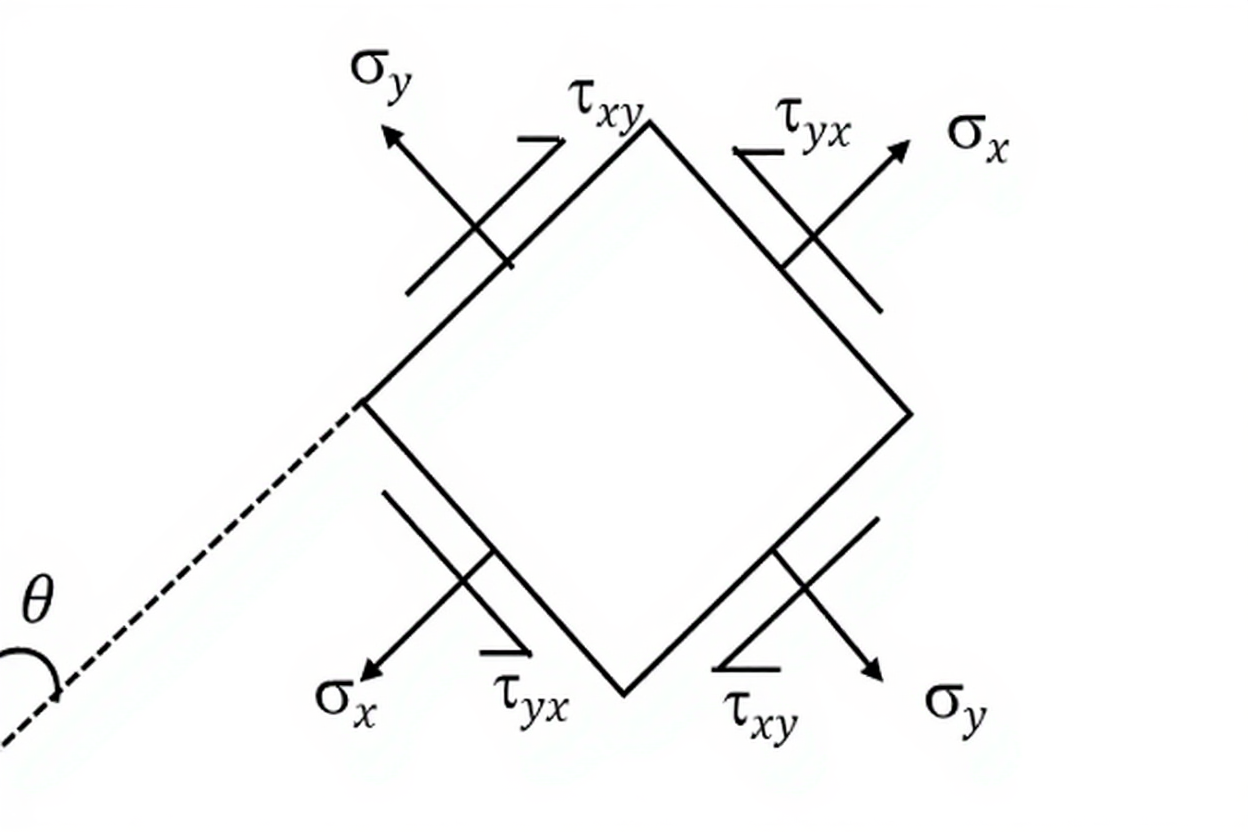
\includegraphics[width=0.4\columnwidth]{figs/fig-21.png}
    \caption*{Fig-21:Rectangular plate with in-plane loads}
    \label{fig-21}
\end{figure}

\end{enumerate}

\begin{enumerate}[itemsep=1em]
\setcounter{enumi}{60}
\item A ship of $5000$ tonnes displacement has a rectangular tank $6$ m long and $10$ m wide, half-filled with oil of relative density $0.8$. The virtual reduction in the transverse 
metacentric height of the ship due to free surface effect of the oil in the tank is \underline{\hspace{2cm}} cm.  
\end{enumerate}

\newpage
\vspace*{0.25cm}

\begin{enumerate}[itemsep=1em]
\setcounter{enumi}{61}
\item An ocean wave of period $8$ s and height $2$ m is propagating in the Indian Ocean from south to north. According to linear wave theory, for the wave to be considered as a 
deep-water wave, the minimum water depth should be \underline{\hspace{1cm}} m (rounded off to the nearest integer). 
    
\end{enumerate}

\begin{enumerate}[itemsep=1em]
\setcounter{enumi}{62}
\item Consider a gas turbine combustor with air as the working fluid. The flow enters the device at $500$ K and leaves at $1400$ K with a mass flow rate of $0.1\,kg/s$. The changes 
in kinetic energy and potential energy of the flow are neglected. Assuming $C_V=0.717 \,kJ/kg-K$ and $R = 0.287\,kJ/kg-K$, the rate of heat addition is \underline{\hspace{1cm}} kW 
(rounded off to the nearest integer). 
\end{enumerate}

\begin{enumerate}[itemsep=1em]
\setcounter{enumi}{63}
\item Consider a circular cylinder of diameter $0.5 \,m$ and length $2\,m$, rotating in clockwise direction at a speed of $100$ rpm in a flow of velocity $2 \,m/s$. Assume the density of the fluid as $1.225\,kg/m^3$ and $\pi= 3.14$. By Kutta-Joukowski theorem, the lift force on the cylinder is \underline{\hspace{2cm}} N (rounded off to the nearest integer). 
\end{enumerate}

\begin{enumerate}[itemsep=1em]
\setcounter{enumi}{64}
\item A new absolute temperature scale is proposed based on a Carnot engine operating between hot and cold reservoirs of temperatures $T_L$ and $T_H$ respectively. Let $Q_L$ and  
$Q_H$ be the respective heat transfers, with the relation given by $\frac{T_L}{T_H}=\frac{Q_L}{Q_H}$. On the new scale, the difference between the steam and ice points of water is $500$ units and the efficiency of the engine is $0.268$.The steam point of water on this scale is \underline{\hspace{1cm}} units.
(rounded off to the nearest integer)
\end{enumerate}





\end{document}
